
    
    
    
    


    


    
    \title{(some) LaTeX environments \par for Jupyter notebook}\author{@jfbercher}

    \section{Introduction}\label{introduction}

    This extension for IPython 4.x or Jupyter enables to use some LaTeX
commands and environments in the notebook's markdown cells.
\begin{enumerate} \item \textbf{LaTeX commands and environments}
\begin{itemize} \item support for some LaTeX commands within
markdown cells, \emph{e.g.} \texttt{\textbackslash{}textit},
\texttt{\textbackslash{}textbf}, \texttt{\textbackslash{}underline},
\texttt{author}, \texttt{\textbackslash{}title}, LaTeX comments \item
support for \textbf{theorems-like environments}, support for labels and
\textbf{cross references} \item support for \textbf{lists}:
\emph{enumerate, itemize},\\
\item limited support for a \textbf{figure environment}, \item support
for an environment \emph{listing}, \item additional \emph{textboxa}
environment \end{itemize} \item \textbf{Citations and
bibliography} \begin{itemize} \item support for
\texttt{\textbackslash{}cite} with creation of a References section
\end{itemize} \item it is possible mix markdown and LaTeX
markup \item \textbf{Document-wide numbering of equations and
environments, support for \texttt{\textbackslash{}label} and
\texttt{\textbackslash{}ref}} \item \textbf{Configuration toolbar} \item
\textbf{LaTeX\_envs dropdown menu for a quick insertion of environments}
\item Support for \textbf{User \LaTeX definitions file} \item
Environments title/numbering can be customized by users in
\texttt{user\_envs.json} config file \item \textbf{Export to HTML and
LaTeX with a customized exporter} \item Styles can be customized in the
\texttt{latex\_env.css} stylesheet \end{enumerate}

A simple illustration is as follows: one can type the following in a
markdown cell

\begin{listing}
The dot-product is defined by equation (\ref{eq:dotp}) in theorem \ref{theo:dotp} just below:
\begin{theorem}[Dot Product] \label{theo:dotp}
Let $u$ and $v$ be two vectors of $\mathbb{R}^n$. The dot product can be expressed as
\begin{equation}
\label{eq:dotp}
u^Tv = |u||v| \cos \theta,
\end{equation}
where $\theta$ is the angle between $u$ and $v$ ...
\end{theorem}
\end{listing}

and have it rendered as

The dot-product is defined by equation (\ref{eq:dotp}) in theorem
\ref{theo:dotp} just below: \begin{theorem}[Dot Product]
\label{theo:dotp} Let \(u\) and \(v\) be two vectors of
\(\mathbb{R}^n\). The dot product can be expressed as

\begin{equation}
\label{eq:dotp}
u^Tv = |u||v| \cos \theta,
\end{equation}

where \(\theta\) is the angle between \(u\) and \(v\) \ldots{}
\end{theorem}

    \subsection{** What's new **}\label{whats-new}

\textbf{November 2, 2016} - version 1.3.1

\begin{itemize}
\tightlist
\item
  Support for \textbf{user environments configuration} file
  (\texttt{user\_envs.json} in nbextensions/latex\_envs directory). This
  file is included by the html export template.\\
\item
  Support for \textbf{book/report style numbering} of environments, e.g.
  ``Example 4.2'' is example 2 in section 4.
\item
  Support for \texttt{\textbackslash{}author},
  \texttt{\textbackslash{}title}, and \texttt{maketitle}. Author and
  title are saved in notebook metadata, used in html/latex exports. The
  maketitle command also formats a title in the LiveNotebook.\\
\item
  Added a Toogle menu in the config toolbar to:

  \begin{itemize}
  \tightlist
  \item
    toggle use of user's environments config file
  \item
    toggle \texttt{report-style} numbering
  \end{itemize}
\end{itemize}

\textbf{September 18, 2016} - version 1.3

\begin{itemize}
\tightlist
\item
  Support for \textbf{user personal LaTeX definitions} file
  (\texttt{latexdefs.tex} in current directory). This file is included
  by the html and latex export templates.\\
\item
  Style for nested enumerate environments added in
  \texttt{latex\_envs.css}
\item
  Added a Toogle menu in the config toolbar to:

  \begin{itemize}
  \tightlist
  \item
    toggle the display of the LaTeX\_envs dropdown menu,
  \item
    toggle the display of labels keys,
  \item
    toggle use of user's LaTeX definition file
  \end{itemize}
\item
  \textbf{Cross references now use the true environment number instead
  of the reference//label key}. \textbf{References are updated
  immediately}. This works \textbf{document wide} and works for pre and
  post references
\item
  Support for optional parameters in theorem-like environments
\item
  Support for spacings in textmode, eg \texttt{\textbackslash{}par},
  \texttt{\textbackslash{}vspace,\ \textbackslash{}hspace}
\item
  Support for LaTeX comments % in markdown cells
- Reworked
  loading and merging of system/document configuration parameters
\end{itemize}

\textbf{August 28, 2016} - version 1.2

\begin{itemize}
\item
  \textbf{Added support for nested environments of the same type}.
  Nesting environments of different type was already possible, but there
  was a limitation for nesting environments of the same kind; eg itemize
  in itemize in itemize. This was due to to the fact that regular
  expressions are not suited to recursivity. I have developped a series
  of functions that enable to extract nested environments and thus cope
  with such situations.
\item
  Corrected various issues, eg
  \href{https://github.com/ipython-contrib/jupyter_contrib_nbextensions/issues/731}{\#731},
  \href{https://github.com/ipython-contrib/jupyter_contrib_nbextensions/issues/720}{\#720}
  where the content of nested environments was incorrectly converted to
  markdown.
\item
  Completely reworked the configuration toolbar. Re-added tips.
\item
  Added a toggle-button for the LaTeX\_envs menu
\item
  Added system parameters that can be specified using the
  \href{https://github.com/Jupyter-contrib/jupyter_nbextensions_configurator/tree/master/src/jupyter_nbextensions_configurator/static/nbextensions_configurator}{nbextensions\_configurator}.
  Thus reworked the configuration loading/saving.
\item
  Reworked extension loading. It now detects if the notebook is fully
  loaded before loading itself.
\end{itemize}

\textbf{August 03, 2016} - version 1.13

\begin{itemize}
\item
  Added a template to also keep the toc2 features when exporting to
  html:

\begin{verbatim}
jupyter nbconvert --to html_toclenvs FILE.ipynb
\end{verbatim}
\item
  Added a dropdown menu that enables to insert all main LaTeX\_envs
  environments using a simple click. Two keybards shortcuts (Ctrl-E and
  Ctrl-I) for equations and itemize are also provided. More environments
  and shortcuts can be added in the file \texttt{envsLatex.js}.
\item
  Added a link in the general help menu that points to the
  documentation.
\end{itemize}

\textbf{July 27, 2016} - version 1.1

\begin{itemize}
\item
  In this version I have reworked \textbf{equation numbering}. In the
  previous version, I used a specialized counter and detected equations
  rendering for updating this counter. Meanwhile, this feature has been
  introduced in \texttt{MathJax} and now we rely on MathJax
  implementation. rendering is significantly faster. We still have keep
  the capability of displaying only equation labels (instead of
  numbers). The numbering is automatically updated and is document-wide.
\item
  I have completely reworked the \textbf{notebook conversion} to plain
  \LaTeX and html. We provide specialized exporters, pre and post
  processors, templates. We also added entry-points to simplify the
  conversion process. It is now as simple as

\begin{Shaded}
\begin{Highlighting}[]
\KeywordTok{jupyter} \NormalTok{nbconvert --to html_with_lenvs FILE.ipynb}
\end{Highlighting}
\end{Shaded}

  to convert \texttt{FILE.ipynb} into html while keeping all the
  features of the \texttt{latex\_envs} notebook extension in the
  converted version.
\end{itemize}

    \section{Main features}\label{main-features}

\subsection{Implementation principle}\label{implementation-principle}

The main idea is to override the standard Markdown renderer in order to
add a \emph{small} parsing of LaTeX expressions and environments. This
heavily uses regular expressions. The LaTeX expression are then rendered
using an html version. For instance
\texttt{\textbackslash{}underline\ \{something\}} is rendered as
\texttt{\textless{}u\textgreater{}\ something\ \textless{}/u\textgreater{}},
that is \underline{something}. The environments are replaced by an html
tag with a class derived from the name of the environment. For example,
a \texttt{definition} denvronment will be replaced by an html rendering
corresponding to the class \texttt{latex\_definition}. The styles
associated with the different classes are specified in
\texttt{latex\_env.css}. These substitutions are implemented in
\texttt{thsInNb4.js}.

    \subsection{Support for simple LaTeX
commands}\label{support-for-simple-latex-commands}

    We also added some LaTeX commands (e.g. \texttt{\textbackslash{}textit},
\texttt{\textbackslash{}textbf}, \texttt{\textbackslash{}underline}) --
this is useful in the case of copy-paste from a LaTeX document. The
extension also supports some textmode spacings, namely
\texttt{\textbackslash{}par},
\texttt{\textbackslash{}vspace,\ \textbackslash{}hspace} as well as
\texttt{\textbackslash{}title}, \texttt{\textbackslash{}author},
\texttt{maketitle} and LaTeX comments \% in markdown cells. Labels and
cross-references are supported, including for equations.

    \subsection{Available environments}\label{available-environments}

    \begin{itemize}
\tightlist
\item
  \textbf{theorems-like environments}: \emph{property, theorem, lemma,
  corollary, proposition, definition,remark, problem, exercise,
  example},
\item
  \textbf{lists}: \emph{enumerate, itemize},\\
\item
  limited support for a \emph{figure} environment,
\item
  an environment \emph{listing},
\item
  \emph{textboxa}, wich is a \texttt{textbox} environment defined as a
  demonstration (see below).
\end{itemize}

More environments can be added easily in the user\_envs config file
\texttt{user\_envs.json} or directly in the javascript source file
\texttt{thmsInNb4.js}. The rendering is done according to the stylesheet
\texttt{latex\_env.css}, which can be customized.
\begin{remark} When exporting to html, the
\texttt{latex\_env.css} file honored is the file on the github CDN.
However, customized css can be added in a \texttt{custom.css} file that
must reside in the same directory as the notebook itself. The reason for
that is that the \texttt{css} file must be in the same directory as the
notebook file for inclusion, which means copying it in each working
directory. As the rendering of the html file obtained is done using the
original javascript code, the same is true for the source files;
therefore it is better to curstomize environments in
\texttt{user\_envs.json} which is taken into account when exporting to
html.\\
\end{remark}

    \subsection{Automatic numerotation, labels and
references}\label{automatic-numerotation-labels-and-references}

    Several counters for numerotation are implemented: counters for problem,
exercise, example, property, theorem, lemma, corollary, proposition,
definition, remark, and figure are available. Mathjax-equations with a
label are also numbered document-wide. An anchor is created for any
label which enables to links things within the document:
\texttt{\textbackslash{}label} and \texttt{\textbackslash{}ref} are both
supported. A limitation was that numbering was updated (incremented)
each time a cell is rendered. Document-wide automatic updating is
implemented since version 1.3. A toolbar button is provided to reset the
counters and refresh the rendering of the whole document (this is still
useful for citations and bibliography refresh).

    \label{example:mixing} A simple example is as follows, featuring
automatic numerotation, and the use of labels and references. Also note
that standard markdown can be present in the environment and is
interpreted. \emph{The rendering is done according to the stylesheet
\texttt{latex\_env.css}, which of course, can be customized to specific
uses and tastes}.

\begin{listing}
\begin{definition} \label{def:FT}
Let $x[n]$ be a sequence of length $N$. Then, its **Fourier transform** is given by
\begin{equation}
\label{eq:FT}
X[k]= \frac{1}{N} \sum_{n=0}^{N-1} x[n] e^{-j2\pi \frac{kn}{N}}
\end{equation}
\end{definition}
\end{listing}

\begin{definition} \label{def:FT} Let \(x[n]\) be a sequence of
length \(N\). Then, its \textbf{Fourier transform} is given by

\begin{equation}
\label{eq:FT2}
X[k]= \frac{1}{N} \sum_{n=0}^{N-1} x[n] e^{-j2\pi \frac{kn}{N}}
\end{equation}

\end{definition}

    It is now possible to refer to the definition and to the equation by
their labels, as in:

\begin{listing}
As an example of Definition \ref{def:FT}, consider the Fourier transform (\ref{eq:FT2}) of a pure cosine wave given by
$$
x[n]= \cos(2\pi k_0 n/N),
$$
where $k_0$ is an integer. 
\end{listing}

    As an example of Definition \ref{def:FT}, consider the Fourier transform
(\ref{eq:FT2}) of a pure cosine wave given by \[
x[n]= \cos(2\pi k_0 n/N),
\] where \(k_0\) is an integer. Its Fourier transform is given by \[
X[k] = \frac{1}{2} \left( \delta[k-k_0] + \delta[k-k_0] \right), 
\] modulo \(N\).

    \subsection{Bibliography}\label{bibliography}

    \subsubsection{Usage}\label{usage}

    It is possible to cite bibliographic references using the standard LaTeX
\texttt{\textbackslash{}cite} mechanism. The extension looks for the
references in a bibTeX file, by default \texttt{biblio.bib} in the same
directory as the notebook. The name of this file can be modified in the
configuration toolbar. It is then possible to cite works in the
notebook, e.g.

\begin{listing}
The main paper on IPython is definitively \cite{PER-GRA:2007}. Other interesting references are certainly \cite{mckinney2012python, rossant2013learning}. Interestingly, a presentation of the IPython notebook has also be published recently in Nature \cite{shen2014interactive}.
\end{listing}

The main paper on IPython is definitively \cite{PER-GRA:2007}. Other
interesting references are certainly
\cite{mckinney2012python, rossant2013learning}. Interestingly, a
presentation of the IPython notebook has also be published recently in
Nature \cite{shen2014interactive}.

    \subsubsection{Implementation}\label{implementation}

    The implemention uses several snippets from the nice
\href{https://bitbucket.org/ipre/calico/downloads/}{icalico-document-tools}
extension that also considers the rendering of citations in the
notebook. We also use a modified version of the
\href{https://code.google.com/p/bibtex-js/}{bibtex-js} parser for
reading the references in the bibTeX file. The different functions are
implemented in \texttt{bibInNb4.js}. The rendering of citations calls
can adopt three styles (Numbered, by key or apa-like) -- this can be
selected in the configuration toolbar. It is also possible to customize
the rendering of references in the reference list. A citation template
is provided in the beginning of file \texttt{latex\_envs.js}:

\begin{verbatim}
var cit_tpl = {
// feel free to add more types and customize the templates
    'INPROCEEDINGS': '%AUTHOR:InitialsGiven%, ``_%TITLE%_\'\', %BOOKTITLE%, %MONTH% %YEAR%.',
    ... etc
\end{verbatim}

The keys are the main types of documents, eg inproceedings, article,
inbook, etc. To each key is associated a string where the \%KEYWORDS\%
are the fields of the bibtex entry. The keywords are replaced by the
correponding bibtex entry value. The template string can formatted with
additional words and effects (markdown or LaTeX are commands are
supported)

    \subsection{Figure environment}\label{figure-environment}

    Finally, it is sometimes useful to integrate a figure within a markdown
cell. The standard markdown markup for that is
\texttt{!{[}link{]}(image)}, but a limitation is that the image can not
be resized, can not be referenced and is not numbered. Furthermore it
can be useful for re-using existing code. Threfore we have added a
limited support for the \texttt{figure} environment. This enables to do
something like

\begin{listing}
\begin{figure}
\centerline{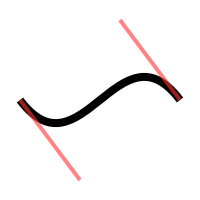
\includegraphics[width=10cm]{example.png}}
\caption{\label{fig:example} This is an example of figure included using LaTeX commands.}
\end{figure}
\end{listing}

which renders as

\begin{figure}
\centerline{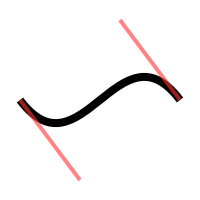
\includegraphics[width=10cm]{example.png}}
\caption{\label{fig:example} This is an example of figure included using LaTeX commands.}
\end{figure}

Of course, this Figure can now be referenced:

\begin{listing}
Figure \ref{fig:example} shows a second filter with input $X_2$, output $Y_2$  and an impulse response denoted as $h_2(n)$
\end{listing}

Figure \ref{fig:example} shows a second filter with input \(X_2\),
output \(Y_2\) and an impulse response denoted as \(h_2(n)\)

    \subsection{figcaption}\label{figcaption}

    For Python users, we have added in passing a simple function in the
\texttt{latex\_envs.py} library.

This function can be imported classically, eg
\texttt{from\ latex\_envs.latex\_envs\ import\ figcaption} (or
\texttt{from\ jupyter\_contrib\_nbextensions.nbconvert\_support.latex\_envs\ import\ figcaption}
if you installed from the jupyter\_contrib repo).

Then, this function enables to specify a caption and a label for the
next plot. In turn, when exporting to \LaTeX, the corresponding plot is
converted to a nice figure environement with a label and a caption.
%
\begin{lstlisting}
%matplotlib inline
import matplotlib.pyplot as plt
from jupyter_contrib_nbextensions.nbconvert_support.latex_envs import figcaption
from numpy import pi, sin, arange

plt.plot(sin(2*pi*0.01*arange(100)))
\end{lstlisting}%
    
    

    
    
    
    \begin{verbatim}
[<matplotlib.lines.Line2D at 0x7f8a1872ba20>]
    \end{verbatim}

    

    
\begin{figure}[H]
\centering
\includegraphics[width=0.6\linewidth]{latex_env_doc_files/latex_env_doc_23_2.png}
\caption{This is a nice sine wave}
\label{fig:mysin}
\end{figure}
%    { \hspace*{\fill} \\}
    
    \subsection{Other features}\label{other-features}

    \begin{itemize}
\item
  As shown in the examples, eg \ref{example:mixing} (or just below),
  \textbf{it is possible to mix LaTeX and markdown markup in
  environments}
\item
  Support for \textbf{line-comments}: lines beginning with a % will
  be masked when rendering 
- Support for \textbf{linebreaks}:
  \texttt{\textbackslash{}par\_}, where \_ denotes any space, tab,
  linefeed, cr, is replaced by a linebreak
\item
  Environments can be nested. egg:

  \begin{listing}
  This is an example of nested environments, with equations inside\\
  \begin{proof} Demo
  % This is a comment
\begin{enumerate}
  \item $$ \left\{ p_1, p_2, p_3 \ldots p_n \right\} $$
  \item A **nested enumerate**
  \item second item 
  \begin{enumerate}
  \item $ \left\{ p_1, p_2, p_3 \ldots p_n \right\} $
  \item And *another one*
  \item second item 
  \begin{enumerate}
  \item $$ \left\{ p_1, p_2, p_3 \ldots p_n \right\} $$
  \item second item 
  \end{enumerate}
  \end{enumerate}
  \end{enumerate}
  \end{proof}
  \end{listing}

  which results in
\end{itemize}

    This is an example of nested environments, with equations inside\\
\begin{proof} Demo % This is a
comment
\begin{enumerate} \item

\begin{equation}\label{eq:}
\left\{ p_1, p_2, p_3 \ldots p_n \right\}
\end{equation}

\[ \left\{ p_1, p_2, p_3 \ldots p_n \right\} \] \item A \textbf{nested
enumerate} \item second item \begin{enumerate} \item
\(\left\{ p_1, p_2, p_3 \ldots p_n \right\}\) \item And \emph{another
one} \item second item \begin{enumerate} \item
\[ \left\{ p_1, p_2, p_3 \ldots p_n \right\} \] \item second item
\end{enumerate} \end{enumerate} \end{enumerate}
\end{proof}

    \subsection{User interface}\label{user-interface}

    \subsubsection{Buttons on main toolbar}\label{buttons-on-main-toolbar}

    On the main toolbar, the extension provides three buttons
\includegraphics{main_toolbar.png} The first one can be used to refresh
the numerotation of equations and references in all the document. The
second one fires the reading of the bibliography bibtex file and creates
(or updates) the reference section. Finally the third one is a toogle
button that opens or closes the configuration toolbar.

    \subsubsection{Configuration toolbar}\label{configuration-toolbar}

    The configuration toolbar \includegraphics{config_toolbar.png} enables
to enter some configuration options for the extension.

First, the \texttt{LaTeX\textbackslash{}\_envs} title links to this
documentation. Then, the bibliography text input can be used to indicate
the name of the bibtex file. If this file is not found and the user
creates the reference section, then this section will indicate that the
file was not found. The \texttt{References} drop-down menu enables to
choose the type of reference calls. The Equations input box enables to
initiate numbering of equations at the given number (this may be useful
for complex documents in several files/parts). The \texttt{Equations}
drop-down menu let the user choose to number equation or to display
their label instead. The two next buttons enable to toogle display of
the LaTeX\_envs environments insertion menu or to toggle the displau of
LaTeX labels. Finally The \texttt{Toogles} dropdown menu enable to
toogle the state of several parameters. All these configuration options
are then stored in the notebook's metadata (and restored on reload).

    The \texttt{Toggles} dropdown menu \includegraphics{Toggles.png}

enables to toggle the state of several configuration options:

\begin{itemize}
\tightlist
\item
  display the \texttt{LaTeX\_envs} insertion menu or not,
\item
  show labels anchors,
\item
  use \LaTeX user own LaTeX defintions (loads \texttt{latexdefs.tex}
  file from current document directory),
\item
  load user's environments configuration (file \texttt{user\_envs.json}
  in \texttt{nbextensions/latex\_envs} directory),
\item
  select ``report style'' numbering of environments
\end{itemize}

    \subsection{\texorpdfstring{The \texttt{LaTeX\_envs} insertion
menu}{The LaTeX\_envs insertion menu}}\label{the-latexux5fenvs-insertion-menu}

The \texttt{LaTeX\_envs} insertion menu
\includegraphics{LaTeX_envs_menu.png} enables a quick insertion of LaTeX
environments, some with a keyboard shorcut (this can be customized in
\texttt{envsLatex.js}). Besides, selected text will be inserted in the
environment.

    \section{Conversion to LaTeX and
HTML}\label{conversion-to-latex-and-html}

    The extension works in the live-notebook. Since it relies on a bunch of
javascript, the notebook does not render as is in services such as
\texttt{nbviewer} or \texttt{github} viewer. Similarly,
\texttt{nbconvert} does not know of the LaTeX constructs which are used
here and therefore does not fully convert notebooks using this
extension.

Therefore, we provide specialized templates and exporters to achieve
these conversions.

    \subsection{Conversion to html}\label{conversion-to-html}

We provide a template \texttt{latex\_envs.tpl} and an exporter class
\texttt{LenvsHTMLExporter} (in library \texttt{latex\_envs.py}). Using
that class, conversion simply amounts to

\begin{verbatim}
jupyter nbconvert --to latex_envs.LenvsHTMLExporter FILE.ipynb
\end{verbatim}

A shortcut is also provided

\begin{verbatim}
jupyter nbconvert --to html_with_lenvs FILE.ipynb
\end{verbatim}

It should be noted that the rendering is done exactly in the same way as
in the livenotebook. Actually, it is the very same javascript which is
run in the html file. The javascript functions are available on the
extension github as well as in the
\texttt{jupyter\_notebook\_extensions} CDN, which means that the
rendering of the html files requires an internet connection (this is
also true for the rendering of equations with MathJax).

Another template \texttt{latex\_envs\_toc.tpl} is provided which enables
to also keep the toc2 features when exporting to html (\emph{it even
works if you do not have the \texttt{toc2} extension!}):

\begin{Shaded}
\begin{Highlighting}[]
\KeywordTok{jupyter} \NormalTok{nbconvert --to html_with_toclenvs FILE.ipynb}
\end{Highlighting}
\end{Shaded}

\textbf{If you use the version included in the
jupyter\_notebook\_extensions collection}, the entry-points (conversion
shortcuts) are a little different: use instead

\begin{itemize}
\item
\begin{verbatim}
jupyter nbconvert --to html_lenvs FILE.ipynb
\end{verbatim}
\item
\begin{verbatim}
jupyter nbconvert --to html_toclenvs FILE.ipynb
\end{verbatim}
\end{itemize}

\subsection{Conversion to LaTeX}\label{conversion-to-latex}

We provide two templates \texttt{thmsInNb\_article.tplx} and
\texttt{thmsInNb\_report.tplx} for article and report styles
respectively. Anyway one can also use the standard article, report, book
templates provided with nbconvert. Simply, we have improved some of the
internals styles. More importantly, we provide an exporter class
\texttt{LenvsLatexExporter} (also in library \texttt{latex\_envs.py}).
Using that class, conversion simply amounts to

\begin{verbatim}
jupyter nbconvert --to latex_envs.LenvsLatexExporter FILE.ipynb
\end{verbatim}

A shortcut is also provided

\begin{verbatim}
jupyter nbconvert --to latex_with_lenvs FILE.ipynb
\end{verbatim}

In addition, we provide several further options:

\begin{itemize}
\tightlist
\item
  \textbf{removeHeaders}: Remove headers and footers, (default false)
\item
  \textbf{figcaptionProcess}: Process figcaptions, (default true)
\item
  \textbf{tocrefRemove} Remove tocs and ref sections, + some cleaning,
  (default true),
\end{itemize}

These options can be specified on the command line as, eg,

\begin{verbatim}
jupyter nbconvert --to latex_with_lenvs --LenvsLatexExporter.removeHeaders=True -- LenvsLatexExporter.tocrefRemove=False FILE.ipynb
\end{verbatim}

\textbf{If you use the version included in the
jupyter\_notebook\_extensions collection}, the entry-points (conversion
shortcuts) are a little different: use instead

\begin{verbatim}
jupyter nbconvert --to latex_lenvs FILE.ipynb
\end{verbatim}

    \begin{example} As for an example, the present document has
been converted using

\begin{verbatim}
jupyter nbconvert --to latex_with_lenvs --LenvsLatexExporter.removeHeaders=True latex_env_doc.ipynb
\end{verbatim}

Then the resulting file (without header/footer) has been included in the
main file \texttt{documentation.tex}, where some LaTeX definitions of
environments are done (namely listings, colors, etc) and compiled using

\begin{itemize}
\tightlist
\item
  \texttt{xelatex\ -interaction=nonstopmode\ documentation}
\item
  \texttt{bibTeX\ documentation}
\item
  \texttt{xelatex\ -interaction=nonstopmode\ documentation}
\end{itemize}

The output can be consulted \href{documentation.pdf}{here}.\\
\end{example}

    \section{Installation}\label{installation}

    The extension consists in a package that includes a javascript notebook
extension. Since Jupyter 4.2, this is the recommended way to distribute
nbextensions. The extension can be installed

\begin{itemize}
\tightlist
\item
  from the master version on the github repo (this will be always the
  most recent version)
\item
  via pip for the version hosted on Pypi
\item
  as part of the great
  \href{https://github.com/ipython-contrib/Jupyter-notebook-extensions}{Jupyter-notebook-extensions}
  collection. Follow the instructions there for installing. Once this is
  done, you can open a tab at
  \texttt{http://localhost:8888/nbextensions} to enable and configure
  the various extensions.
\end{itemize}

From the github repo or from Pypi,

\begin{itemize}
\tightlist
\item
  \textbf{step 1}: install the package

  \begin{itemize}
  \tightlist
  \item
    \texttt{pip3\ install\ https://github.com/jfbercher/jupyter\_latex\_envs/archive/master.zip\ {[}-\/-user{]}{[}-\/-upgrade{]}}
  \item
    { or}
    \texttt{pip3\ install\ jupyter\_latex\_envs\ {[}-\/-user{]}{[}-\/-upgrade{]}}
  \item
    { or} clone the repo and install
    \texttt{git\ clone\ https://github.com/jfbercher/jupyter\_latex\_envs.git\ \ \ \ python3\ setup.py\ install}
  \end{itemize}
\end{itemize}

With Jupyter \textgreater{}= 4.2,

\begin{itemize}
\item
  \textbf{step 2}: install the notebook extension

\begin{verbatim}
jupyter nbextension install --py latex_envs [--user]
\end{verbatim}
\item
  \textbf{step 3}: and enable it

\begin{verbatim}
jupyter nbextension enable latex_envs [--user] --py
\end{verbatim}
\end{itemize}

For Jupyter versions before 4.2, the situation is more tricky since you
will have to find the location of the source files (instructions from
@jcb91 found
\href{https://github.com/jcb91/jupyter_highlight_selected_word}{here}):
execute

\begin{verbatim}
python -c "import os.path as p; from jupyter_highlight_selected_word import __file__ as f, _jupyter_nbextension_paths as n; print(p.normpath(p.join(p.dirname(f), n()[0]['src'])))"
\end{verbatim}

Then, issue

\begin{verbatim}
jupyter nbextension install <output source directory>
jupyter nbextension enable latex_envs/latex_envs
\end{verbatim}

where \texttt{\textless{}output\ source\ directory\textgreater{}} is the
output of the python command.

    \section{Customization}\label{customization}

\subsection{Configuration parameters}\label{configuration-parameters}

Some configuration parameters can be specified system-wide, using the
\texttt{nbextension\_configurator}. For that, open a browser at
\url{http://localhost:8888/nbextensions/} -- the exact address may
change eg if you use jupyterhub or if you use a non standard port. You
will then be able to change default values for the boolean values -
LaTeX\_envs menu (insert environments) present - Label equation with
numbers (otherwise with their \label{} key) - Number environments as
section.num - Use customized environments as given in `user\_envs.json'
(in the extension directory) and enter a default filename for the bibtex
file (in document directory).

All these values can also be changed per documents and these values are
stored in the notebook's metadata.

\subsection{User environments
configuration}\label{user-environments-configuration}

Environments can be customized in the file \texttt{user\_envs.json},
located in the \texttt{nbextensions/latex\_envs} directory. It is even
possible to add \emph{new} environments. This file is read at startup
(or when using the corresponding toggle option in the \texttt{Toggles}
menu) and merged with the standard configuration. An example is provided
as \texttt{example\_user\_envs.json}. For each (new/modified)
environment, one has to provide (i) the name of the environment (ii) its
title (iii) the name of the associated counter for numbering it; eg

\begin{verbatim}
    "myenv": {
        "title": "MyEnv",
        "counterName": "example"
    },
\end{verbatim}

Available counters are problem, exercise, example, property, theorem,
lemma, corollary, proposition, definition, remark, and figure.

\subsection{Styling}\label{styling}

The document title and the document author (as specified by
\texttt{\textbackslash{}title} and \texttt{\textbackslash{}author} are
formatted using the \texttt{maketitle} command according to the
\texttt{.latex\_maintitle} and \texttt{.latex\_author} div styles.

Each environment is formatted according to the div style
\texttt{.latex\_environmentName}, e.g. \texttt{.latex\_theorem},
\texttt{.latex\_example}, etc. The titles of environments are formatted
with respect to \texttt{.latex\_title} and the optional parameter wrt
\texttt{.latex\_title\_opt}. Images are displayed using the style
specified by \texttt{.latex\_img} and thir caption using
\texttt{.caption}. Finally, enumerate environments are formatted
according to the \texttt{.enum} style. Similarly, itemize environments
are formatted using \texttt{.item} style.

These styles can be customized either in the \texttt{latex\_envs.css}
file, or better in a \texttt{custom.css} in the document directory.

    \section{Usage and further examples}\label{usage-and-further-examples}

    \subsection{First example (continued)}\label{first-example-continued}

    We continue the first example on fthe Fourier transform definition
\ref{def:FT} in order to show that, of course, we can illustrate things
using a simple code. Since the Fourier transform is an essential tool in
signal processing, We put this in evidence using the \texttt{textboxa}
environment -- which is defined here in the css, and that one should
define in the LaTeX counterpart:

\begin{listing}
\begin{textboxa}
The Fourier transform is an extremely useful tool to have in your toolbox!
\end{textboxa}
\end{listing}

    \begin{textboxa}
The Fourier transform is an extremely useful tool to have in your toolbox!
\end{textboxa}

    The Fourier transform of a pure cosine is given by \[
X[k] = \frac{1}{2} \left( \delta[k-k_0] + \delta[k-k_0] \right), 
\] modulo \(N\). This is illustrated in the following simple script:
%
\begin{lstlisting}
%matplotlib inline
import numpy as np
import matplotlib.pyplot as plt 
from numpy.fft import fft
k0=4; N=128; n=np.arange(N); k=np.arange(N)
x=np.sin(2*np.pi*k0*n/N)
X=fft(x)
plt.stem(k,np.abs(X))
plt.xlim([0, 20])
plt.title("Fourier transform of a cosine")
_=plt.xlabel("Frequency index (k)")
\end{lstlisting}%
    \begin{center}
    \adjustimage{max size={0.6\linewidth}{0.6\paperheight}}{latex_env_doc_files/latex_env_doc_46_0.png}
    \end{center}
%    { \hspace*{\fill} \\}
    
    \subsection{Second example}\label{second-example}

    This example shows a series of environments, with different facets;
\textbf{links, references, markdown or/and LaTeX formatting within
environments}. The listing of environments below is typed using the
environment \emph{listing}\ldots{}

    \begin{listing}
\begin{definition} \label{def:diffeq}
We call \textbf{difference equation} an equation of the form
$$
\label{eq:diffeq}
y[n]= \sum_{k=1}^{p} a_k y[n-k] + \sum_{i=0}^q b_i x[n-i]
$$
\end{definition}

\begin{property}
If all the $a_k$ in equation (\ref{eq:diffeq}) of definition \ref{def:diffeq} are zero, then the filter has a **finite impulse response**. 
\end{property}

\begin{proof}
Let $\delta[n]$ denote the Dirac impulse. Take $x[n]=\delta[n]$ in (\ref{eq:diffeq}). This yields, by definition, the impulse response:
$$
\label{eq:fir}
h[n]= \sum_{i=0}^q b_i \delta[n-i],
$$
which has finite support. 
\end{proof}

\begin{theorem}
The poles of a causal stable filter are located within the unit circle in the complex plane.
\end{theorem}

\begin{example} \label{ex:IIR1}
Consider $y[n]= a y[n-1] +  x[n]$. The pole of the transfer function is $z=a$. The impulse response $h[n]=a^n$ has infinite support.
\end{example}

In the following exercise, you will check that the filter is stable iff $a$<1.

\begin{exercise}\label{ex:exofilter}
Consider the filter defined in Example \ref{ex:IIR1}. Using the **function** `lfilter` of scipy, compute and plot the impulse response for several values of $a$.
\end{exercise}

\end{listing}

    The lines above are rendered as follows (of course everything can be
tailored in the stylesheet): %
\begin{definition}
\label{def:diffeq} We call \textbf{difference equation} an equation of
the form

\begin{equation}
\label{eq:diffeq}
y[n]= \sum_{k=1}^{p} a_k y[n-k] + \sum_{i=0}^q b_i x[n-i]
\end{equation}

\end{definition} %
Properties of the filter are linked to
the coefficients of the difference equation. For instance, an immediate
property is %
% this is a comment
\begin{property}
If all the \(a_k\) in equation (\ref{eq:diffeq}) of definition
\ref{def:diffeq} are zero, then the filter has a \textbf{finite impulse
response}. \end{property} %
\begin{proof} Let
\(\delta[n]\) denote the Dirac impulse. Take \(x[n]=\delta[n]\) in
(\ref{eq:diffeq}). This yields, by definition, the impulse response:

\begin{equation}
\label{eq:fir}
h[n]= \sum_{i=0}^q b_i \delta[n-i],
\end{equation}

which has finite support. \end{proof}
%
\begin{theorem} The poles of a causal stable filter are
located within the unit circle in the complex plane.
\end{theorem} %
\begin{example} \label{ex:IIR1}
Consider \(y[n]= a y[n-1] + x[n]\). The pole of the transfer function is
\(z=a\). The impulse response \(h[n]=a^n\) has infinite support.
\end{example}

In the following exercise, you will check that the filter is stable iff
\(a\)\textless{}1. %
\begin{exercise}\label{ex:exofilter}
Consider the filter defined in Example \ref{ex:IIR1}. Using the
\textbf{function} \texttt{lfilter} of scipy, compute and plot the
impulse response for several values of \(a\). \end{exercise}

    \begin{listing}
The solution of exercise \ref{ex:exofilter}, which uses a difference equation as in Definition \ref{def:diffeq}:
\end{listing}

The solution of exercise \ref{ex:exofilter}, which uses a difference
equation as in Definition \ref{def:diffeq}:
%
\begin{lstlisting}
%matplotlib inline
import numpy as np
import matplotlib.pyplot as plt 
from scipy.signal import lfilter
d=np.zeros(100); d[0]=1 #dirac impulse
alist=[0.2, 0.8, 0.9, 0.95, 0.99, 0.999, 1.001, 1.01]
for a in alist:
    h=lfilter([1], [1, -a],d)
    _=plt.plot(h, label="a={}".format(a))
plt.ylim([0,1.5])
plt.xlabel('Time')
_=plt.legend()
\end{lstlisting}%
    \begin{center}
    \adjustimage{max size={0.6\linewidth}{0.6\paperheight}}{latex_env_doc_files/latex_env_doc_52_0.png}
    \end{center}
%    { \hspace*{\fill} \\}
    
    \subsection{Third example:}\label{third-example}

    This example shows that environments like itemize or enumerate are also
available. As already indicated, this is useful for copying text from a
TeX file. Following the same idea, text formating commands
\texttt{\textbackslash{}textit}, \texttt{\textbackslash{}textbf},
\texttt{\textbackslash{}underline}, etc are also available.

    \begin{listing}
The following \textit{environments} are available:
\begin{itemize}
    \item \textbf{Theorems and likes}
    \begin{enumerate}
        \item theorem,
        \item lemma,
        \item corollary
        \item ...
    \end{enumerate}
    \item \textbf{exercises}
    \begin{enumerate}
        \item problem,
        \item example,
        \item exercise
    \end{enumerate}
\end{itemize}
\end{listing}

    which gives\ldots{}

The following \textit{environments} are available:
\begin{itemize} \item \textbf{Theorems and likes}
\begin{enumerate} \item theorem, \item lemma, \item corollary \item
\ldots{} \end{enumerate} \item \textbf{exercises}
\begin{enumerate} \item problem, \item example, \item exercise
\end{enumerate} \end{itemize}

    \section{Disclaimer, sources and
thanks}\label{disclaimer-sources-and-thanks}

    Originally, I used a piece of code from the nice online markdown editor
\texttt{stackedit}
\url{https://github.com/benweet/stackedit/issues/187}, where the authors
also considered the problem of incorporating LaTeX markup in their
markdown.

I also studied and used examples and code from
\url{https://github.com/ipython-contrib/IPython-notebook-extensions}.

\begin{itemize}
\item
  This is done in the hope it can be useful. However there are many
  impovements possible, in the code and in the documentation.
  \textbf{Contributions will be welcome and deeply appreciated.}
\item
  If you have issues, please post an issue at
  \texttt{https://github.com/jfbercher/jupyter\_latex\_envs/issues}
  \href{https://github.com/jfbercher/jupyter_latex_envs/issues}{here}.
\end{itemize}

\textbf{Self-Promotion --} Like \texttt{latex\_envs}? Please star and
follow the
\href{https://github.com/jfbercher/jupyter_latex_envs}{repository} on
GitHub.

    